\chapter{Úvod}

Práce se zabývá vytvořením hry pro více hráčů a využitím umělé inteligence pro naprogramování umělých hráčů pro tuto hru. Cílem nebylo pouze vytvořit novou hru, ale především se zamyslet nad tím, jak naprogramovat umělou inteligenci ve hře, jejíž stav se velice rychle mění.

% Stav hry totiž nezávisí pouze na pohybu protivníků. V~závislosti na tom, jak si hráč ve hře vede, se také mění jeho velikost a rychlost, což znamená, že pro něj v~různých situacích budou otevřeny různé cesty nebo jedním pohybem se v~různých situacích posune o~různou vzdálenost. Právě ten fakt, že ... činí z~této práce jistou výzvu.

V~práci je nejdříve popsána teorie týkající se umělé inteligence. Popsána je základní teorie nutná pro pochopení fungování umělých hráčů a~následně algoritmy, které tito umělí hráči využívají.

V~další sekci je popsána hra samotná bez detailů o~implementaci. Stanoveny jsou pravidla hry, její ovládání, menu, různé funkce, a~také se zmiňuje o~hrách, které inspirovaly její vytvoření.

Následuje sekce implementační; využité knihovny, navigace mezi různými menu a~pohledy, popis fungování hry samotné a~zlehka je zde popsána implementace umělé inteligence ve hře.

Zjednodušenou verzi této hry jsem již dříve vytvořil v jazyce \emph{Scratch}. Princip hry byl v~mnoha ohledech stejný; hlavním rozdílem je absence umělých hráčů. V~závěru práce bude výsledek této práce porovnán s~původní verzí hry. \todo{Good idea?}


\chapter{Umělá inteligence ve hře}

Tato kapitola se zabývá nejdříve umělou inteligencí a~jejím využitím ve hrách obecně, poté se zaměřuje na její využití v tomto projektu.


\section{Umělá inteligence}

Umělá inteligence je rozsáhlá vědní disciplína z~oboru informačních technologií. Existuje řada různých definic, které se liší v~tom, jak na umělou inteligenci nahlíží. Některé ji vnímají jako proces rozhodování, zatímco jiné jako chování. Některé nahlíží na napodobování lidského chování, jiné na rozumnost chování. Obecně by se dalo o~umělé inteligenci hovořit jako o~napodobování inteligence přirozené, nicméně ani inteligence samotná nemá jasnou definici.

Existuje také řada zaměření umělé inteligence. Mezi typická zaměření patří například:
\begin{itemize}
    \item řešení úloh,
    \item strojové učení,
    \item plánování a~rozhodování,
    \item reprezentace znalostí,
    \item počítačové vidění
\end{itemize}
a~jiné. Zaměřením této práce je především \uv{řešení úloh} \todo{a~\uv{plánování a~rozhodování}?}.


\section{Řešení úloh}

V~oblasti umělé inteligence je řešením úlohy nalezení posloupnosti kroků od počátečního stavu k~cílovému stavu. Cílové stavy mohou být popsány explicitně (např. v~případě \uv{Hanojských věží}) nebo podmínkami, které musí být splněny (např. \uv{šach mat} ve hře Šachy).
\todo{Obrázky: Hanojské věže, Šachy}

\subsection*{Úlohy}

Úlohu lze formálně definovat pěticí komponent \cite{AI_Russel_Norvig}:
\begin{itemize}
    \item Počáteční stav úlohy.
    \item Množina operátorů, které slouží pro přechod mezi stavy úlohy. U~některých úloh nelze v~každém stavu aplikovat kterýkoliv operátor.
    \item Množina následníků jednotlivých stavů, kterých lze dosáhnout aplikací určitých operátorů. Jedná se o~funkci se 2~operandy: ${Succ(s, a)}$. Jejím výsledkem je stav, do něhož se přejde po aplikaci operátoru $a$ na stav $s$.
    \item Množina cílových stavů. Jak bylo zmíněno, lze je popsat explicitním výčtem cílových stavů nebo pomocí omezujících podmínek.
    \item Nezáporné ceny přechodů mezi stavy. Tato komponenta je opět funkce -- ${c(s, a, s')}$, jejíž výsledkem je cena vykonání přechodu ze stavu $s$ do stavu $s'$ pomocí operátoru $a$. Některé metody řešení úloh tuto cenu nezohledňují. Zpravidla platí, že čím nižší cena, tím kvalitnější řešení.
\end{itemize}
Pomocí této formální definice lze pak řešení definovat jako nalezení posloupnosti operátorů, jejichž postupnou aplikací se z~počátečního stavu dosáhne jednoho z~množiny cílových stavů.

Prostředí úlohy umělé inteligence musí být plně pozorovatelné, deterministické, statické a~diskrétní. Aby bylo prostředí plně pozorovatelné, musí být kdykoliv možné zjistit jeho úplný stav. Aby bylo deterministické, pak aplikací jednoho operátoru na jeden stav musí být pokaždé učiněn stejný přechod. Statické prostředí se nesmí měnit svévolně; změna musí být vždy výsledkem provedení přechodu.

\subsection*{Metody řešení}

Pro řešení úloh existuje řada metod. Výběr metody může zásadně ovlivnit dobu hledání řešení i~jeho optimálnost. Nejde pouze o~kvalitu vybrané metody, ale také o~to, zda se pro danou úlohu hodí vybranou metodu použít.

Při řešení úlohy pomocí umělé inteligence je bezpodmínečně nutné určit cílové stavy a~operátory, a~také jakým způsobem může být použití některých operátorů v~některých stavech omezeno. Pomocí použité metody se pak na základě dostupných operátorů budou hledat nové stavy a~provádět kontrola, zda nebylo dosaženo stavu cílového.

S~tímto také souvisí pojem abstrakce. Abstrakcí se myslí zahrnutí pouze těch vlivů, které jsou důležité pro danou úlohu a~ignorování těch, které na řešení nemají vliv. Například, pokud hledáme nejkratší cestu autem z~Brna do Prahy, nemusí nás zajímat, kolik lidí v~autě pojede. Dobrá abstrakce se může projevit na době hledání řešení, avšak přílišná abstrakce se může příliš odchýlit od skutečného problému a~přinést výsledky, které na něj nelze aplikovat.

Jsou úlohy, u~kterých není relevantní kvalita řešení, ale pouze splnění určitých podmínek, úlohy, kde je kvalita určena počtem vykonaných kroků, a úlohy, kde je kvalita určena cenami vykonaných přechodů. Proto může být někdy nutné správně určit ceny přechodů mezi stavy, nebo alespoň faktory, které mají na cenu přechodu vliv. V~tom případě je však vhodné zvolit metodu, která ceny přechodů bere v~úvahu.

Úlohy jsou hodnoceny podle těchto kritérií:
\begin{itemize}
    \item Úplnost -- Pokud má daná úloha řešení, pak ho metoda vždy najde.
    \item Optimálnost -- Pokud existuje více řešení dané úlohy, pak metoda najde vždy to nejlepší.
    \item Časová náročnost -- Jak bude růst čas hledání řešení s~rostoucí komplexností zadání.
    \item Prostorová náročnost -- Jak se budou zvyšovat požadavky na paměť s~rostoucí komplexností zadání.
\end{itemize}

Pro reprezentaci časové a prostorové náročnosti se většinou používá Landauova notace (notace omikron). V~ní často figuruje hloubka stromu a~tzv. \uv{faktor větvení}, což je průměrný počet bezprostředních následníků při expanzi uzlu.

\todo{Dělení -- prohledávání stavového prostoru, CSP, hraní her, lok. prohledávání, rozklad na podproblémy, ...?}


\section{Řešení úloh prohledáváním stavového prostoru}

Prohledávání stavového prostoru je jedním z~několika přístupů k~řešení úloh pomocí umělé inteligence. Stavový prostor lze chápat jako vyhledávací strom\footnote{\uv{Vyhledávací strom} je datová struktura. Z~hlediska teorie grafů se jedná o~\uv{zakořeněný orientovaný strom}.}, kde uzly představují stavy řešení úlohy a~hrany představují aplikaci vybraného operátoru na daný stav. Kořenem tohoto stromu je pak výchozí stav úlohy.

Častým problémem těchto vyhledávacích stromů je opakování stavů. Jelikož u~některých úloh je možné dosáhnout stavu, který se již ve vyhledávacím stromu nachází, může pak nastat situace, že se některé stavy budou opakovat stále dokola. V~takovém případě je daný strom nekonečný. Spousta metod však dokáže s~takovými stromy pracovat a~nebo generují strom tak, aby opakování stavů předešly.

Při řešení úlohy není nutné konstruovat celé stromy a~pak v~nich hledat cesty od kořene k~cílovým stavům. Algoritmu většinou stačí prozkoumat jen část stavového prostoru, aby nalezl cílový stav. Postup řešení většinou začíná u~stromu, který má pouze 1 uzel --- počáteční stav --- a~ten se následně \emph{expanduje}. \emph{Expanzí} se myslí vygenerování nových stavů pro každý operátor aplikovatelný na daný stav. Nově vygenerované uzly se dále expandují do té doby, než je nalezen cílový stav. (Nutno podotknout, že může nastat i~situace, kdy cílový stav bude sám stav počáteční, a~tedy k~žádné expanzi nedojde.)

Základem metod, které využívají přístupu prohledávání stavového prostoru, je algoritmus \emph{Tree search}. Samotné metody se pak většinou liší pouze ve strategii výběru uzlu pro expanzi. Algoritmus využívá kolekci\footnote{V~literatuře \todo{zdroj} se často uvádí datový typ \uv{seznam}, avšak to by znamenalo, že prvky v~této struktuře musí být seřazeny. Obecně pro fungování algoritmu stačí, aby struktura podporovala operace vkládání a~vyjímání a~nezáleží na pořadí, v~němž jsou prvky vyjímány.} OPEN pro uchování uzlů určených k~expanzi. Princip fungování algoritmu lze popsat pomocí pseudokódu:
\begin{enumerate}
    \item Inicializuj kolekci OPEN, aby obsahovala pouze počáteční uzel.
    \item Pokud je kolekce OPEN prázdná, ukonči prohledávání jako \underline{neúspěšné}. Jinak pokračuj na další bod.
    \item Vyber a~vyjmi jeden uzel z~kolekce OPEN.
    \item Pokud je vybraný uzel uzlem cílovým, ukonči prohledávání jako \underline{úspěšné}. Jinak pokračuj na další bod.
    \item Expanduj vybraný uzel -- všechny jeho bezprostřední následníky vlož do kolekce OPEN.
    \item Vrať se na bod 2.
\end{enumerate}
\todo{FIXME?: Kolekce, kontejner nebo seznam after all?}
\todo{FIXME?: Má cenu popisovat Tree search bez CLOSED?}

Jak bylo zmíněno, ve vyhledávacích stromech se často opakují stejné stavy, což má za důsledek nekonečné stromy. V~takovém případě by mohlo nastat, že algoritmus \emph{Tree search} se nikdy nezastaví. Tento problém lze vyřešit drobnou úpravou algoritmu. Upravený algoritmus bude využívat ještě jednu kolekci --- kolekci CLOSED --- do níž se budou vkládat uzly, které již byly expandovány. Pseudokód pro \emph{Tree search} s~kolekcí CLOSED vypadá pak takto (nově přidané části jsou zvýrazněny tučně):
\begin{enumerate}
    \item Inicializuj kolekci OPEN, aby obsahovala pouze počáteční uzel.
    \textbf{\item Inicializuj kolekci CLOSED jako prázdnou}.
    \item Pokud je kolekce OPEN prázdná, ukonči prohledávání jako \underline{neúspěšné}. Jinak pokračuj na další bod.
    \item Vyber a~vyjmi jeden uzel z~kolekce OPEN \textbf{a~vlož jej do kolekce CLOSED}.
    \item Pokud je vybraný uzel uzlem cílovým, ukonči prohledávání jako \underline{úspěšné}. Jinak pokračuj na další bod.
    \item Expanduj vybraný uzel -- všechny jeho bezprostřední následníky, \textbf{kteří nejsou v~kolekci OPEN ani CLOSED,} vlož do kolekce OPEN.
    \item Vrať se na bod 3.
\end{enumerate}
Kromě přidání nové kolekce se rozšířila i~funkce kolekce OPEN -- obě dvě nyní plní funkci množiny všech stavů, které jsou součástí aktuální podoby stavového prostoru (kolekce OPEN však stále plní funkci uchovávání stavů určených k~expanzi).

Pokud nestačí pouze najít cílový stav, ale také posloupnost kroků, která k~němu vedou, je nutná rekonstrukce cesty. U~\emph{Tree search} je rekonstrukce cesty poměrně jednoduchá -- stačí si u~každého uzlu uložit jeho bezprostředního předchůdce. Po nalezení cílového stavu se pak rekonstrukce provede tak, že se rekurzivně budou hledat předchůdci cílového uzlu v~kolekci CLOSED, dokud není nalezen počáteční stav.

Základní rozdělení metod, které řeší úlohy prohledáváním stavového prostoru, je rozdělení na neinformované a informované. Rozdíl mezi nimi je v~tom, že neinformované nemají žádnou informaci o~vztahu mezi libovolným stavem a~stavem cílovým kromě toho, zda tento stav cílový je nebo není. Tím pádem tyto metody nemají žádné prostředky k~tomu, aby mohly stavy nějakým způsobem hodnotit a~vybírat si pro expanzi uzly, které jsou řešení blíže než ostatní. Neinformovanými metodami však není třeba se zde zabývat, neboť v~práci použity nejsou. \todo{Popsat i~blind search nebo ne?}

Informované metody mají k~dispozici informace o~cílovém stavu a~dokážou s~těmito informacemi pracovat, aby optimalizovaly hledání cesty stromem. Společný algoritmus pro informované metody se nazývá \emph{Best-first search} (zkr. \emph{BestFS}). Tento algoritmus vychází z~algoritmu \emph{Tree search}; my si zde ukážeme pouze variantu s~kolekcí CLOSED:
\begin{enumerate}
    \item Inicializuj kolekci OPEN, aby obsahovala pouze počáteční uzel.
    \item Inicializuj kolekci CLOSED jako prázdnou.
    \item Pokud je kolekce OPEN prázdná, ukonči prohledávání jako \underline{neúspěšné}. Jinak pokračuj na další bod.
    % The `\textbf` isn't enough to make the equation bold.
    \item Vyber a vyjmi uzel ${s_k}$ \textbf{s~nejnižším ohodnocením \boldmath${f(s_k)}$} z~kolekce OPEN a~vlož jej do kolekce CLOSED
    \item Pokud je vybraný uzel uzlem cílovým, ukonči prohledávání jako \underline{úspěšné}. Jinak pokračuj na další bod.
    \item Expanduj vybraný uzel -- všechny jeho bezprostřední následníky, kteří nejsou v~kolekci OPEN ani CLOSED, vlož do kolekce OPEN.
    \item Vrať se na bod 3.
\end{enumerate}

Konkrétní metody se pak liší v~tom, jakým způsobem se vypočítá hodnota ${f(s_k)}$. Ve~výpočtech vždy figuruje tzv. heuristická funkce ${h(s_k)}$ -- odhad ceny nejlevnější cesty z~uzlu ${s_k}$ k~cílovému uzlu. Výpočet ${h(s_k)}$ se neváže ke konkrétní metodě; metody samotné pouze mohou definovat podmínky, které tato funkce musí splňovat. Jedinou podmínkou, která musí platit vždy, je, že pokud $s_k$ je cílový uzel, pak ${h(s_k) = 0}$.

\begin{figure}
    \centering
    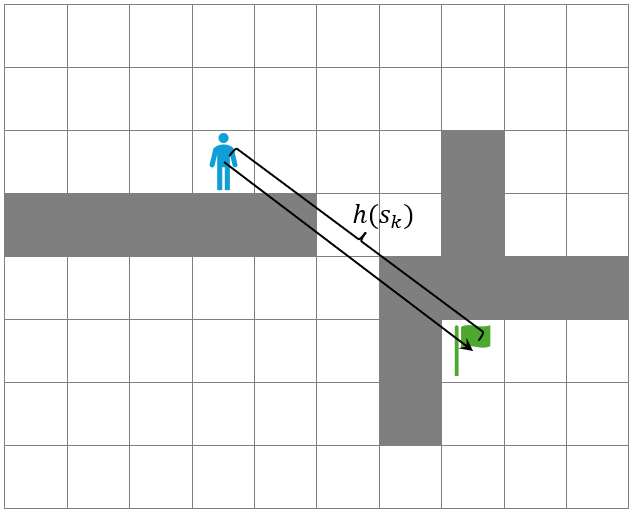
\includegraphics[height=7cm]{doc/obrazky-figures/informed-heuristic-example.png}
    \caption{Příklad heuristické funkce. Úkolem je najít cestu labyrintem. Jako heuristika byla vybrána přímá vzdálenost mezi středy aktuální a~cílové buňky.}
    \label{fig:informed-heuristic-example}
\end{figure}


\subsection{Metoda A*}

Metoda A* je jedna z~nejrozšířenějších informovaných metod prohledávání stavového prostoru. Pro výpočet využívá jak heuristickou funkci, tak cenu cesty, tedy:
\[f(s_k) = g(s_k) + h(s_k)\]
\begin{figure}
    \centering
    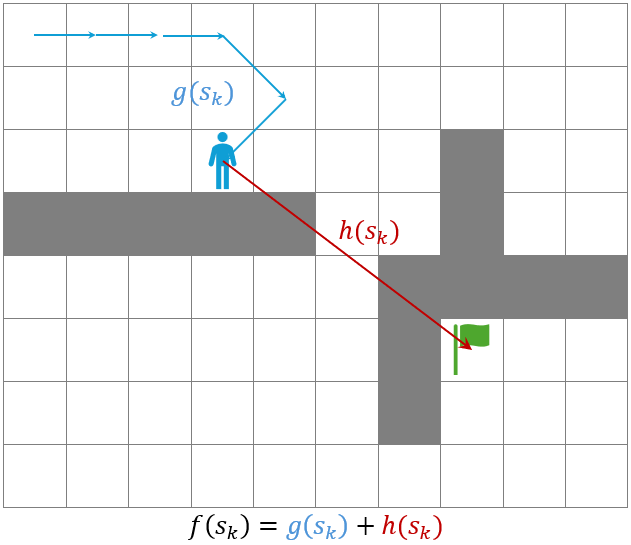
\includegraphics[height=7cm]{doc/obrazky-figures/astar-fsk-example.png}
    \caption{Výpočet hodnoty ${f(s_k)}$ u~metody A*. Světle modrá křivka označuje cestu z~počátečního uzlu, červená odhadovanou cestu k~cílovému uzlu. Ceny přechodů zde nejsou vyznačeny, ale předpokládejme, že cena zvolené cesty z~počátečního k~aktuálnímu uzlu je opravdu nejnižší možná.}
    \label{fig:astar-fsk-example}
\end{figure}

Metoda je úplná i~optimální, avšak pro optimálnost musí heuristická funkce splňovat určité podmínky: musí být přípustná a, v~případě použití seznamu CLOSED, musí být konzistentní. \todo{cite https://dl.acm.org/doi/10.1145/3828.3830}

Aby byla heuristika přípustná, musí být spodním odhadem skutečné cesty od ohodnocovaného uzlu k~cílovému. To znamená, že pro každý uzel $s_k$ musí být ${h(s_k)}$ menší nebo rovna skutečné ceně cesty k~cíli.

Aby byla heuristika konzistentní, pak pro každý uzel $s_k$ a~jeho následníka $s_{k+1}$ generovaného operátorem $a$ musí platit, že odhad ceny cesty z~uzlu $s_k$ k~cíli není větší, než cena přechodu z~$s_k$ do $s_{k+1}$ pomocí operátoru $a$ plus odhad ceny cesty z~uzlu $s_{k+1}$ k~cíli. Popsáno rovnicí:
\[h(s_k) \le c(s_k, a, s_{k+1}) + h(s_{k+1})\]
Jinými slovy, musí být splněna trojúhelníková nerovnost, viz obrázek \ref{fig:astar-heuristic-consistency}.

\begin{figure}
    \centering
    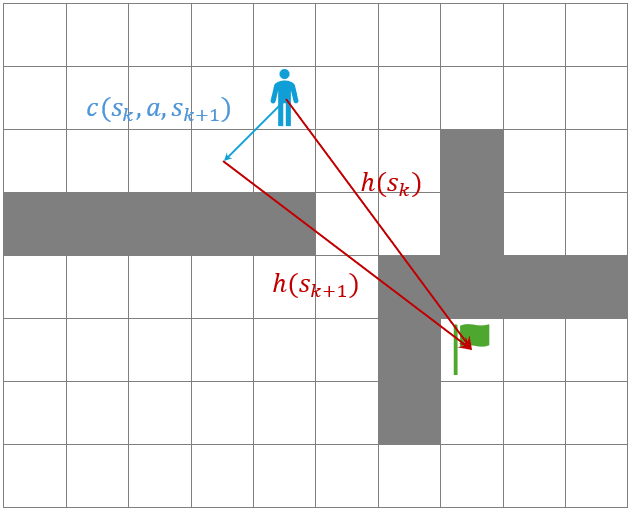
\includegraphics[height=7cm]{doc/obrazky-figures/astar-heuristic-consistency.png}
    \caption{Heuristika $h$ je konzistentní, jelikož platí trojúhelníková nerovnost -- součet délek kterýchkoliv dvou stran musí být větší nebo roven délce strany třetí. Stranami jsou zde ${h(s_k)}$, ${c(s_k, a, s_{k+1})}$ a~${h(s_{k+1})}$}
    \label{fig:astar-heuristic-consistency}
\end{figure}


\chapter{Představení hry}

\section{Pravidla}
Hra je typu \uv{battle royale}. Jejím cílem je tedy eliminovat všechny protivníky a~zůstat poslední naživu. Hráči ovládají kruhové entity nazývané \uv{bubliny} (\uv{bubbles}) ve 2rozměrném labyrintu. 

Hra umožňuje hráčům svislý, vodorovný i~diagonální pohyb. Překážky v~labyrintu jsou vyznačeny polygony, skrz které hráči nemohou procházet. Kromě toho představuje hrací plocha obdélníkový box, který taktéž není možné opustit. Mimo pohybu je možné změnit stav bubliny tím, že hráč (manuálně) zmenší její velikost. Tato možnost existuje z~důvodu, aby bylo možné projít úzkými chodbami, pro které je bublina příliš velká. Důsledkem však je, že hráč takto ztratí body života (viz následující odstavec), nicméně nelze takto ztratit poslední bod života.

Hráči začínají s~určitým množstvím bodů života a~zůstávají ve hře, dokud je toto množství větší než 0. Když se 2 a~více hráčů dotýká, všichni dotýkající se hráči ztrácí body života. Kromě toho na této veličině závisí několik dalších vlastností hráče:
\begin{itemize}
    \item Velikost -- poloměr hráčovy bubliny (přímo úměrně),
    \item Rychlost pohybu (nepřímo úměrně),
    \item Síla -- kolik bodů života ubírá hráč svým protivníkům,
    \item Množství života získaného z~bonusů -- viz dále (nepřímo úměrně).
\end{itemize}

V~průběhu hry se v~náhodných intervalech objevují na hrací ploše bonusy ve tvaru čtverce, které hráčům doplňují body života. Aby byl bonus na hráče aplikován, musí se bonus s~bublinou hráče navzájem dotýkat. Následkem toho tento bonus zmizí a~žádný jiný hráč ho poté už nemůže použít. Místo, kde se bonus objeví je náhodné. Nikdy však nemůže kolidovat s~překážkou, ani se nemůže objevit v~určité vzdálenosti od nějakého hráče nebo jiného bonusu.

\section{Uživatelské rozhraní}

\todo{Vstup z klávesnice}
\todo{Výstup na obrazovku}
    \todo{Hrací plocha}
    \todo{Navigace}

\section{Editor herní plochy}

\section{Podobné hry}
\todo{Agar.io -- player model, contact damage, ...}
\todo{Worms -- bonuses, AI}


\chapter{Implementace}

\section{Použité knihovny}

\subsection*{Simple DirectMedia Layer}

SDL (Simple DirectMedia Layer) je multiplatformní knihovna, která poskytuje nízkoúrovňový přístup ke vstupu z~klávesnice, myši, joysticku, výstupu zvuku a~grafiky. Je napsána v~jazyce C a~funguje nativně i~v~C++. Oficiálně podporuje platformy Windows, macOS, Linux, Android a~iOS. V~projektu je použita verze 2 této knihovny (SDL2).

SDL má také několik přidružených knihoven, které rozšiřují její funkcionalitu. \todo{Satellite libs used in the project}

\subsection*{libSDL2pp}

Knihovna libSDL2pp slouží pro reprezentaci SDL2 a~přidružených knihoven pomocí objektového modelu jazyka C++.

\subsection*{SDL\_gfx}

Knihovna SDL\_gfx slouží pro vykreslení některých základních geometrických tvarů, které SDL v~základu nepodporuje, jako jsou například křivky a~elipsy. Je napsána v~jazyce C a~funguje nativně i~v~C++.


\chapter{Závěr}

\todo{Závěr}
